\subsubsection*{The benefits of Live Interactivity for Uncertainty
  Quantification}

The ability to stop, modify, or restart computations `in flight' has
the potential to significantly improve the efficiency of an
uncertainty analysis. There exist many algorithms, for example
adaptive Markov chain Monte Carlo methods~\parencite{GilksEtal1994}, 
which attempt to choose the best samples based on the sampling
history. For complex problems however, a domain expert
may often have
a better idea about the region of the parameter domain where function
evaluations should be concentrated. Through live programming within a
tight feedback loop a domain expert can incrementally guide the
current sampling strategy being used for uncertainty 
quantification, and in turn be guided by 
real time information derived from the reduced order model 
(such as surpluses
provided by sparse grid approximation to 
identify important parameter dimensions and regions of interest), 
to improve the end result. The resulting strategies are expected to be
more aggressive in nature as they are better targeted to the specific
problem at hand. The result of this is more efficient quantification of
uncertainty.

In this project, by accelerating the feedback loop between
$\mathbf{p}$ and $Q(U_{\mathbf{p}})$, together with estimates of its
uncertainty, we will give the scientist the ability to interactively
\emph{explore} the connection (and the associated uncertainty) between
the different dimensions of $\mathbf{p}$ and the overall response of
the system. By understanding the human-factors and systems-level time
constraints on the delivery of useful information in disaster-response
settings, we will be able to specify timing requirements on our model
simulations. By developing software that is time-constrained and
time-aware, we will be able to provide decision makers with
information when it is needed and with an estimate on the uncertainty
of that information.

%Ultimately, the scientist needs an \textbf{interactive interface} for
%gleaning insights from their models in the presence of these
%challenges.

We will address these three challenges using sparse grids and reduced
basis models combined with live modification of simulation parameters,
dynamic steering of computational resources and interactive
visualisation. Specifically:
\begin{enumerate}
\item \emph{Uncertainty in inputs:} sparse grids and reduced basis models can be used
  to pre-compute a surrogate model, $\mathbf{p} \rightarrow \tilde{U}_{\mathbf{p}}$, of the original
  (expensive) model solution process, $\mathbf{p} \rightarrow {U}_{\mathbf{p}}$.
  The expectation integrals of the original model over subsets of the
  parameter space $\mathcal{P}$ (which are important for quantifying
  uncertainty) can be efficiently estimated from the
  surrogate model. This has
  significant benefits over classical Monte Carlo methods when the
  integrand is sufficiently
  smooth~\parencite{JakemanRoberts2013,FranzelinDiehlPfluger2014}.

\item \emph{Cheap to calculate:} for many problems the computation
  of solutions $U_{\mathbf{p}}(\mathbf{x})$ to the model
  $M_{\mathbf{p}}$ can be done cheaply using the combination technique
  over the domain $\mathbf{x}\in\Omega$. An alternative is to use
  proper orthogonal decompositions or greedy algorithms to construct a
  reduced order model which is cheap to compute. In both
  cases the initial construction can be somewhat costly but the
  savings gained later when these surrogates are used extensively for
  UQ and optimisation significantly outweigh this cost. Additionally,
  the initial construction can be done in an offline phase. For our
  disaster response scenarios, the concept of `cheapness' will be
  re-framed as one of `timeliness'. We will build systems which
  guarantee modelling results within timeframes of
  relevance to human factor processes in group decision making
  (occurring in the online phase).

\item \emph{Easy to interpret:} since a sparse grid sampling of
  $\mathbf{p}\in\mathcal{P}$ enables a fast and efficient exploration
  of parameter space, there is more time for visualisation and
  post-processing in an interactive interface, which facilitates
  richer ensembles of visualisation techniques to assist the
  decision-maker in interpreting the results of the model.
\end{enumerate}

%\begin{figure}
 % \centering
  %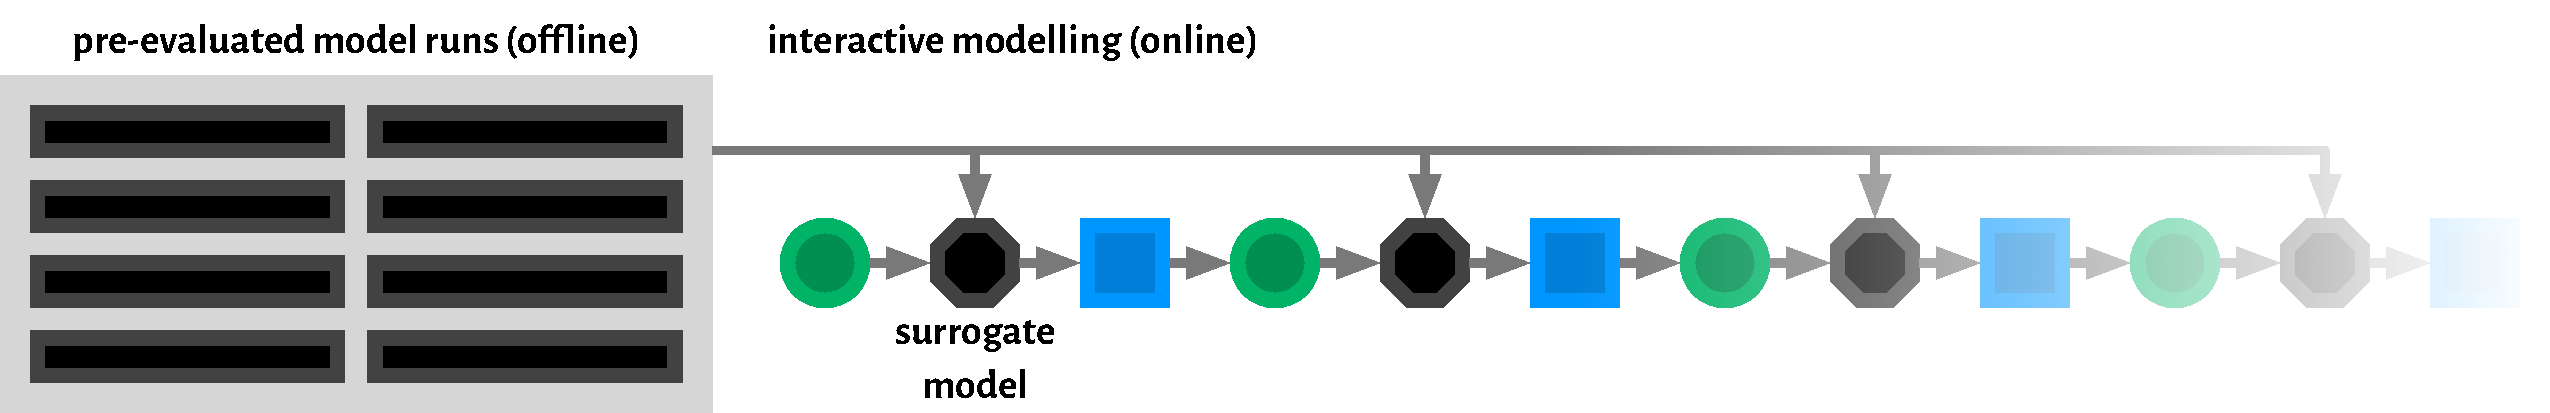
\includegraphics[width=\textwidth]{figures/sg-surrogate-model-fb-loop.pdf}
  %\caption{Using the sparse grids and reduced basis models, the computationally
   % expensive model calculations can be done ahead-of-time and used to
    %construct a surrogate model which can be used to re-claim the
    %interactive workflow of Figure~\ref{fig:unrolled-fb-loop}}.
  %\label{fig:sg-surrogate-model-fb-loop}
%\end{figure}

%Impact: new algorithms, software, high performance computer systems
%and visualisation techniques for time-bound environmental simulation
%with uncertainty. New software tools for the simulation of flood
%surges and tsunami. New methodologies for rapid and agile software
%development and usability using live programming. New knowledge of
%human-in-the-loop requirements for support systems in the context of
%environmental disaster management. New algorithms, software, high
%performance computer systems and visualisation techniques for
%time-bound environmental simulation with uncertainty. New software
%tools for the simulation of flood surges and tsunami. New
%methodologies for rapid and agile software development and usability
%using live programming. New knowledge of human-in-the-loop
%requirements for support systems in the context of environmental
%disaster management.


